\subsection{Overview}
\graphicspath{ {./texfiles/electrical/eimc/} }
%Electrical overview content here
(a) Explain the main requirements and constraints that drive the design. \\
Strict EHW rules \\
reliability \\
reusability \\
lightweight \\
power of pump, valves etc. 

\par Our Low Voltage system drives all electrical and digital control systems of the Fermion. As stated previously,
reliability is crucial in this case. A failure of any component may lead to the shutdown of critical systems, such as the battery management system.
Furthermore, an overvoltage may potentially damage these systems, causing safety hazards. We had the option between building a LV battery pack from spare LiPo cells we ordered for the HV battery pack, and using automotive-grade ventilated lead-acid batteries.
After considering the safety problems of LiPo cells and the efforts of either building a second (smaller) LV BMS or taking the risk of having a singular point of failure by controlling both systems with the same BMS, powering the BMS with the cells it controls, we went for the approach with lead-acid batteries, that is widely used in automotive systems. It is regarded as more reliable and robust compared to the Lithium-Ion pendants that we use for the High Voltage System. \\
\subsubsection*{Power requirements}
We consider the power consumption of all components in the low voltage power line for the power requirements:

( Moussa: Bitte finde die einzelnen Daten heraus. Pumpe ist Pierburg CW150A. Valve ist bei den brakes controllern. Raspberry Pi und Microcontroller passen.)
\begin{itemize}
    \item \textbf{Solenoid Valves:} According to the data sheet, the valves use 2.25 Watts à 4 valves = 9 Watts. While switching, which takes 3.5 ms, they use 8.5 Watts.
    Assuming that we switch all four valves 20 times, we have an additional consumption of \(0.595 J\), which is almost negleglible. We will assume a power consumption of 10 Watts for tolerance.
    \item \textbf{Thermal Pump:} Given the water flow rate, we calculated a theoretical need of 34 Watts for the pump. As we do not have experimental data, we assume that 50 Watts are required at maximum.
    
    \item \textbf{Raspberry Pi 4:} One Raspberry Pi 4B consumes \(10 \, \text{Watts}\).
    \item \textbf{Raspberry Pico W:}
    \item One Raspberry Pico W does not consume more than \(1 \, \text{Watt}\). 

    \item \textbf{Microcontrollers (TIC2000 F280039C):}
    \begin{itemize}
        \item According to datasheet, one microcontroller uses \(3.3V * 0.11 A = 0.363 W \). The controller circuits will not exceed 5 Watts in total. 
    \end{itemize}

    \item \textbf{BMS (Orion BMS 2, 180 Cells):}
       Our BMS consumes up to 2 Watts, according to the datasheet.

    \item \textbf{Leadrive Inverter:} Using the nominal power ratings of 3 A at 24 V, we have a power consumption of 72 Watts.
    \item \textbf{IMD}: Our IMD consumes up to 2 Watts, according to the datasheet.
    \item Network transceiver: We use the Rocket M2, which consumes up to 6 Watt of energy, according to the datasheet.
    \item Precharge relay and contactors: Our precharge relay uses \(0.32 W \), our main contactors use \(2 * 12V * 1A\) in total. We will calculate with 25W.
\end{itemize}

Now, summing up all the power requirements, we have
\(10W + 50W + 10W + 1W + 5W + 2W + 72W + 2W + 6W + 25W = 183W \) , which is roughly 7.7 A at 24V. \\
Using the discharge chart of the data sheet of the LV Battery,
\begin{wrapfigure}{r}{0.25\textwidth}
    \centering
    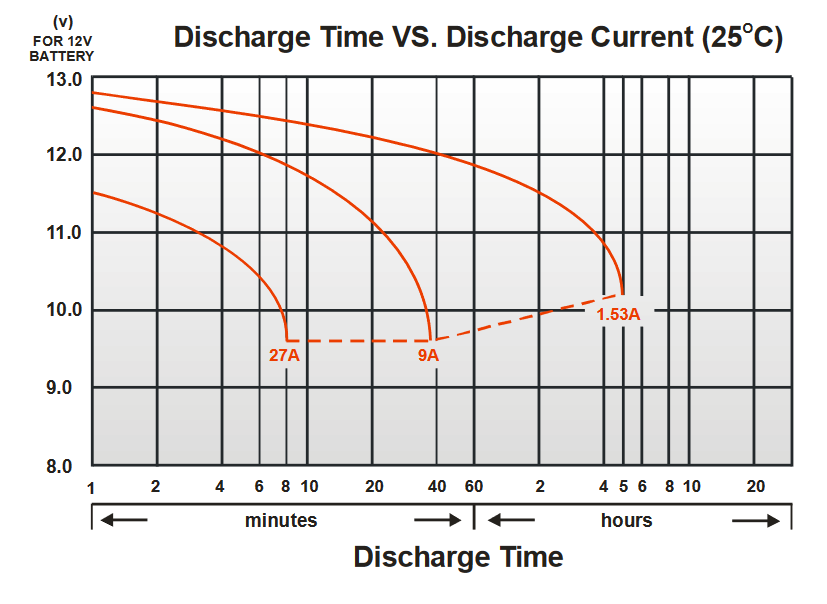
\includegraphics[width=0.25\textwidth]{texfiles/elec/eimg/LV_Battery_WP1236W}
    \caption{Discharge chart of LV battery cell}
\end{wrapfigure}
it is evident that even at full power (9A - including some headroom for losses), we can run our low voltage system for 20 minutes. During the competition, we can rule out that we will use that much power over the whole 20 minutes. 
Assuming that the pump is activated while the HV system is at work, and that this duration takes 2 minutes maximum (the actual run will be much less - max. 20 seconds), and we assume only a usage of 111 W for the rest of the time,
we can use the LV battery for well over 20 minutes. \\
In conclusion, the capacity of 9Ah is a trade-off between the mass and the available runtime of the system.
\subsection{Electrical and mechanical design process}
%Electrical and mechanical design process content here
\subsubsection{Schematic}
\begin{figure}[h]
    \centering
    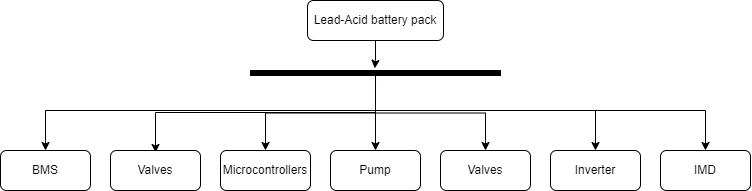
\includegraphics[width=0.75\textwidth]{texfiles/elec/eimg/LV_Diagram}
    \caption{Diagram of LV connections}
\end{figure}
\begin{figure}[h]
    \centering
    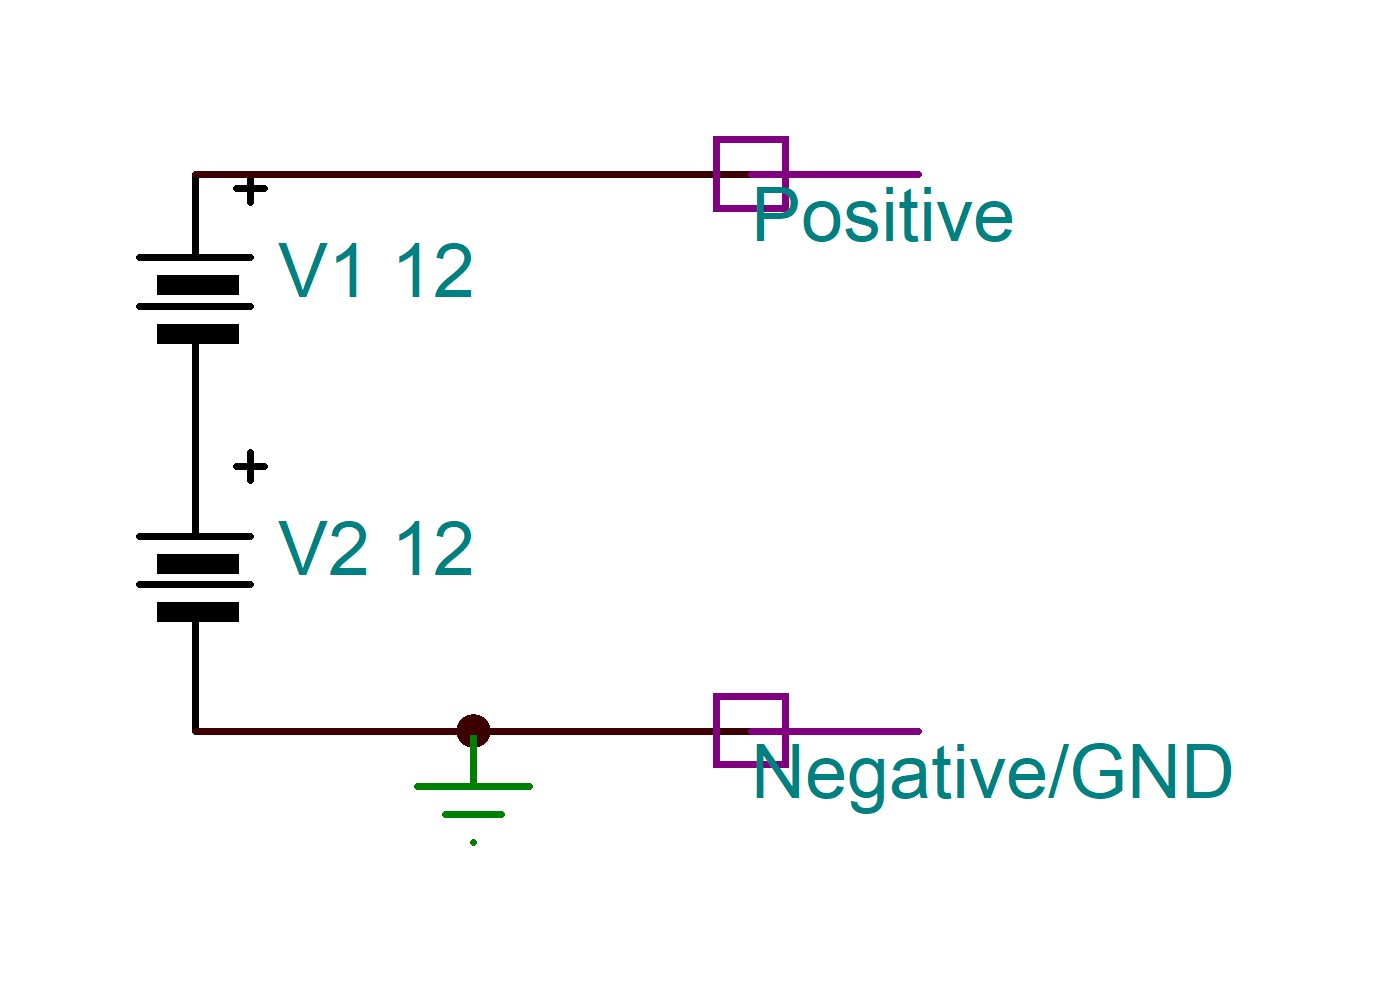
\includegraphics[width=0.5\textwidth]{texfiles/elec/eimg/LVCircuit}
    \caption{Schematic of LV battery cell}
\end{figure}
\subsubsection{(b) Present temperature simulations for vacuum conditions.}
We did a rough estimation based on the internal resistance of the
battery, which is around \(0.014 \Omega \) according to the datasheet. We will assume \(0.02 \Omega\). Using the equation of heat loss, we get \(P = I^2 * R = 8^2 * 0.02 * W = 1.28W\).\\
The ... Bohdan \\


For our heat simulations, we used the software of ANSYS. By vacuum conditions, we assumed the
lack of gas flow, which eliminates the cooling heat flow from winds. The simulation tool solves
the heat transfer equation \( \frac{\partial T}{\partial t} = \alpha \left( \frac{\partial^2 T}{\partial x^2} + \frac{\partial^2 T}{\partial y^2} + \frac{\partial^2 T}{\partial z^2} \right) \)
by discretizing through Finite-Element-Methods.

\subsection{Electrical system characteristics}
%Content of the electrical system characteristics here
\begin{table}[h]
    \centering
    \begin{adjustbox}{width=\textwidth,center}
    \begin{tabular}{|c|c|}
       \hline
       Battery Type & Lead-Acid(integrated)\\
       \hline
       Capacity[Ah] & 9 \\
       \hline
       Nominal Voltage[V] & 12 \\
       \hline
       Cell configuration & 2s \\
       \hline
       Max. discharge [A] & 10 \\
       \hline
       Weight per cell [Kg] & 2,7 \\
       \hline 
       Dimensions per cell (L x W x H)[mm] & 151 x 65 x 94 \\
       \hline 
    \end{tabular}
    \end{adjustbox}
    \label{Low Voltage Cell Specs}
    \caption{LV battery cell characteristics}
\end{table}    

\begin{table}[h]
    \centering
    \begin{adjustbox}{width=\textwidth,center}
    \begin{tabular}{|c|c|}
       \hline
       Battery Type & Lead-Acid(integrated)\\
       \hline
       Capacity[Ah] & 9 \\
       \hline
       Nominal Voltage[V] & 24 \\
       \hline
       Cell configuration & 2s \\
       \hline
       Max. discharge [A] & 10 \\
       \hline
       Weight [Kg] & 5.5 \\
       \hline 
       Dimensions (L x W x H)[mm] & 151 x 65 x 94 \\
       \hline 
    \end{tabular}
    \end{adjustbox}
    \label{Low Voltage Battery Specs}
    \caption{LV battery pack characteristics}
\end{table}    

\subsection{Interface with other system}
%Interface with other system content here n
Briefly reference the communication protocols or control mechanisms of the boards, which should be explained in the respective Sense and Control subsection. \\
All the electric subsystems are located within the pod. \\
It powers the entire sensing, control and telemetry system. 
The LV battery itself does not communicate. Its sensor data is processed by the thermal control board.
When the voltage drops below a certain threshold, the complete system shuts down.

\subsection{Final system description}
%Description of the system here
The two lead-acid batteries, chained in series, provide a nominal voltage of 24V (12V each). When fully charged, the voltage can increase up to 26 V. The lead acid batteries' voltage will drop while discharging. Hence, we monitor the voltage while using the LV battery system. Furthermore, we monitor the temperature through a NTC thermistor to prevent usage under overtemperature . \\
The 24 V power source gets transferred down to 12V (for the Thermal Pump) and 5V for the micro-controllers by buck converters, and drives the valves and several sensors at 24V simultaneously. \\
After reaching out to the EHW technical committee, we were able to clarify that a BMS, used by Lithium-Ion batteries, is not required for lead-acid batteries due to the inherently different chemical structure which makes over- and undercharging much less critical. \\
For charging, we are using a battery charger specified for 12V and 24V lead acid cells from Würth 0510955908. The charging of lead-acid batteries in series is unproblematic, given that we regularly test for drifts and manually balance the cells.\\

\subsection{Manufacturing process}
%Manufacturing process content here
As the cells come in hard-shell covers already, the manufacturing process is not very complicated. We will 3D-print a casing.

\subsection{Testing}
%Testing content here
We will test whether the lead acid cells and the thermistors are accurate to their datasheet. This especially includes \begin{itemize}
    \item the capacity of the packs at 9V discharge (according to real scenario)
    \item the heat development while discharging
\end{itemize}
    %\subsection{FMEA}
%FMEA content here
